\documentclass[letterpaper,11pt,leqno]{article}
\usepackage{paper}
\bibliographystyle{paper}

% Enter paper title to populate PDF metadata:
\hypersetup{pdftitle={Minimalist LaTeX Template for Academic Papers}}

% Enter path to BibTeX file with references:
\newcommand{\bib}{paper.bib}

\begin{document}

% Enter title:
\title{Epistemology}

% Enter authors:
\author{Ibrahim Nasser}

% Enter date:
\date{July 2025}   

% Enter permanent URL (can be commented out):
\available{https://github.com/96ibman/latex-paper/tree/mybranch}

\begin{titlepage}
\maketitle

% Enter abstract:
This is the abstract. Lorem ipsum dolor sit amet, consectetur adipiscing elit, sed do eiusmod tempor incididunt ut labore et dolore magna aliqua. Ut enim ad minim veniam, quis nostrud exercitation ullamco laboris nisi ut aliquip ex ea commodo consequat. Duis aute irure dolor in reprehenderit in voluptate velit esse cillum dolore eu fugiat nulla pariatur. Excepteur sint occaecat cupidatat non proident, sunt in culpa qui officia deserunt mollit anim id est laborum. Lorem ipsum dolor sit amet, consectetur adipiscing elit, sed do eiusmod tempor incididunt ut labore et dolore magna aliqua. Ut enim ad minim veniam, quis nostrud exercitation ullamco laboris nisi ut aliquip ex ea commodo consequat. Duis aute irure dolor in reprehenderit in voluptate velit esse cillum dolore eu fugiat nulla pariatur. Excepteur sint occaecat cupidatat non proident, sunt in culpa qui officia deserunt mollit anim id est laborum. Lorem ipsum dolor sit amet, consectetur adipiscing elit, sed do eiusmod tempor incididunt ut labore et dolore magna aliqua.

\end{titlepage}

% Enter main text:
\section{Introduction}\label{s:introduction}
Sed ut perspiciatis, unde omnis iste natus error sit voluptatem accusantium doloremque laudantium, totam rem aperiam eaque ipsa, quae ab illo inventore veritatis et quasi architecto beatae vitae dicta sunt, explicabo. Nemo enim ipsam voluptatem, quia voluptas sit, aspernatur aut odit aut fugit, sed quia consequuntur magni dolores eos, qui ratione voluptatem sequi nesciunt, neque porro quisquam est, qui dolorem ipsum, quia dolor sit amet consectetur adipiscing velit, sed quia non numquam eius modi tempora incidunt, ut labore et dolore magnam aliquam quaerat voluptatem. 

Sed ut perspiciatis, unde omnis iste natus error sit voluptatem accusantium doloremque laudantium, totam rem aperiam eaque ipsa, quae ab illo inventore veritatis et quasi architecto beatae vitae dicta sunt, explicabo.

\section{Generic section}\label{s:section}

This is a section. This is the section introduction. Below are the subsections.

\subsection{Generic subsection}

Lorem ipsum dolor sit amet, consectetur adipiscing elit. Nulla facilisi. Nullam molestie, libero sit amet luctus vehicula, eros purus ultrices libero, eget fermentum leo sapien a metus. Duis porta massa vel justo posuere, nec placerat neque dictum. Morbi nec velit in turpis fermentum cursus nec ut leo. Integer vitae eros vehicula, fermentum turpis sed, fermentum elit. Suspendisse ac mauris at nisl ultricies commodo id nec justo. 



\subsection{Subsection with references} 

References can be appended at the end of a sentence, in parenthesis \citep{MS15}.  References can be in text: for instance, \citet{M12} found this. It's also possible to collate several references to the same author: for instance, \citet{M12,M14} found things.

It is possible to insert a URL: \url{https://github.com/pmichaillat/latex-paper}.


\section{Section with math}\label{s:math}

This section displays a number of mathematical expressions to showcase the math fonts used in the template.

\subsection{Roman letters} 

The Roman characters in math are just the same as the characters in the text---but in \textit{italic}. Here are some small letters: 
\begin{equation*}
a\{p - r \times l\} + \frac{w(g/z+j)}{i(t)+j(t)+k(t) - e^p - x^j} + \frac{h[f]+x^f}{k[y]-e^y + x^y} = f(j)^{6+y} - i^3_{g,j,p} \approx (p_{ji})^5.
\end{equation*}
Here are some capital letters as well: 
\begin{equation*}
G[p + P^7-Q] - A_B + L\{j\} = F(X) \to [Y+K]\times Z_f/H - [g_4 - i],\;\text{for any}\;i.
\end{equation*}
The punctuation is also the same in math as in text. 


\subsection{Greek letters}

Here are some small Greek letters in a math display: 
\begin{equation*}
\alpha^{\theta} + \gamma^4 + g(a) - \zeta \times \frac{y(\lambda)}{\kappa \cdot k+ \sigma - s} \to \nu_{\eta} = \beta^\epsilon \cdot \delta - \mu + \frac{\xi^4}{\zeta_{ij}} \to m(x) + b^e + \omega .
\end{equation*}
Here are some capital Greek letters in another math display: 
\begin{equation}
F(\Psi) - G(\Phi) \times \Delta^{10} = \Sigma \cdot \Omega^2 - \frac{\Lambda_i}{\Theta_j} \cdot \frac{\Gamma(x)}{\Pi(t)}.
\label{e:capitalgreek}\end{equation}


\subsection{Bold characters}

In the template it is possible to bold all math characters. Roman characters can be bolded, such as $\bm{a} + \bm{D} = \bm{E}^2 + \bm{j}/\bm{i}$. Greek characters can also be bolded, such as $\bm{\alpha} + \bm{\Delta} = \bm{\epsilon}^2 + \bm{\Lambda}/\bm{\Phi}$. It is also possible to bold digits: $1 + 2 \neq \bm{1} + \bm{2}$. Finally, it is possible to bold calligraphic letters: $\bm{\mathcal{C}} + \bm{\mathcal{E}} - [\bm{\mathcal{X}}+\bm{\mathcal{Y}}]$.\footnote{Blackboard-bold letters are already ``bold'' so they cannot be bolded further.}
 

\subsection{Some theorems}

Here is a proposition with some more math:   

\begin{proposition}\label{p:type1}  Lorem ipsum dolor sit amet, consectetur adipiscing elit:
\begin{equation}
\sum_k\bm{S}_{k_x}(z) \approx \frac{S(z)^x}{k / 23 -\zeta\gamma [45- S(z)] + \ln(y) - j^2+x(l)}.
\label{e:type1}\end{equation}
\end{proposition}

\begin{proof} Here is the proof to the proposition. Donec commodo justo a eros malesuada, eget vulputate tortor accumsan. Sed ac pulvinar nulla. Etiam quis felis dapibus, vulputate metus eu, finibus nunc. Sed vel sodales dui. Nam venenatis dolor non orci tempus fermentum. Vivamus sodales justo a ligula cursus aliquet. Sed fringilla nunc vitae justo finibus, id placerat lectus sodales.\end{proof} 

Now here is a lemma:

\begin{lemma}\label{p:cv} Ut enim ad minim veniam, quis nostrud exercitation ullamco laboris nisi ut aliquip ex ea commodo consequat:
\begin{equation}
z^* = \int_{0}^{\infty} \alpha(i) \cdot \frac{1-\beta}{1-\alpha(i)\beta}\,di.
\label{e:cv}\end{equation}
\end{lemma}

And here is a corollary following the lemma:

\begin{corollary} Lorem ipsum dolor sit amet, consectetur adipiscing elit, sed do eiusmod tempor incididunt ut labore et dolore magna aliqua:
\begin{equation*}
\mathbb{E}(N(z^*)) \approx \frac{1-\mathbb{P}(\alpha\pi)}{1-\pi}- \frac{f(y)}{z(p)^*} + P(\Gamma).
\end{equation*}
Ut enim ad minim veniam, quis nostrud exercitation ullamco laboris nisi ut aliquip ex ea commodo consequat.\end{corollary}

\section{Section with graphs}\label{s:graphs}

Here is a section with a variety of graphs.

\subsection{Subsection with graphs at the top of the page}

A simple two-panel graph is on figure \ref{f:graph1}. It will be placed at the top of the page, just about here. Et harum quidem rerum facilis est et expedita distinctio. Nam libero tempore, cum soluta nobis est eligendi optio, cumque nihil impedit, quo minus id, quod maxime placeat, facere possimus, omnis voluptas assumenda est, omnis dolor repellendus. Temporibus autem quibusdam et aut officiis debitis aut rerum necessitatibus saepe eveniet, ut et voluptates repudiandae sint et molestiae non recusandae.

\begin{figure}[h!]
  \centering
  \subcaptionbox{A first panel, 1951--2019\label{f:panel1}}{
    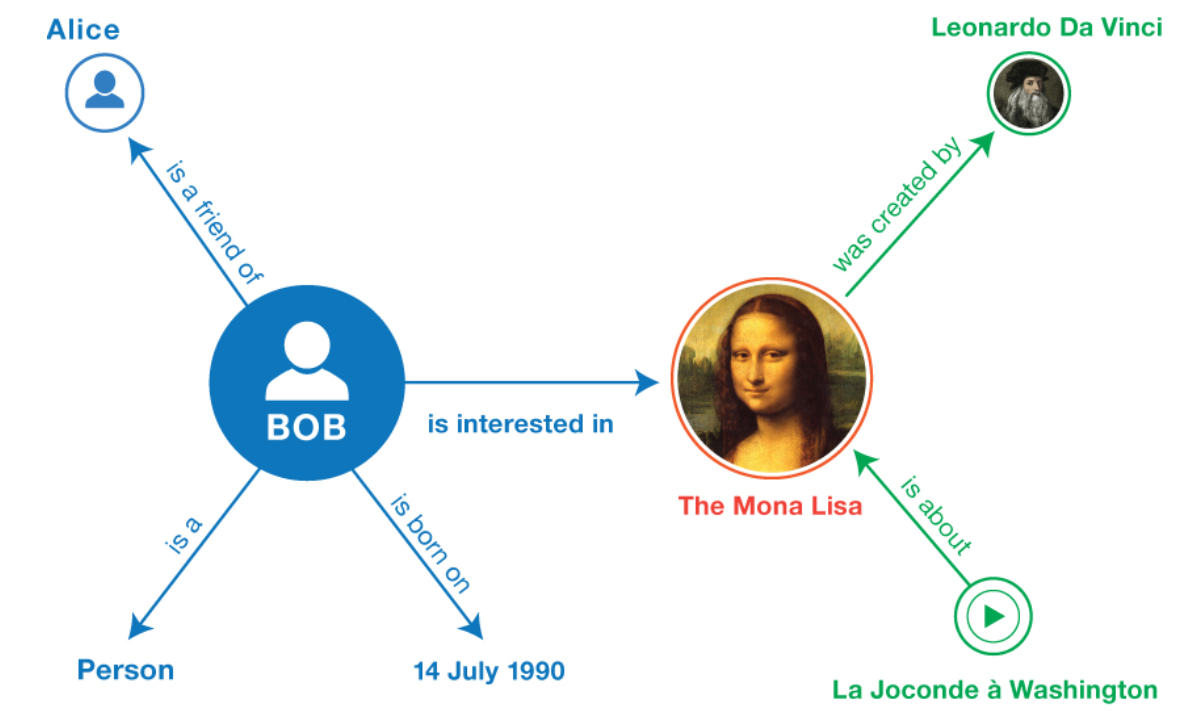
\includegraphics[width=0.45\textwidth]{images/kg.png}
  }\hfill
  \subcaptionbox{A second panel, 1951--2019\label{f:panel2}}{
    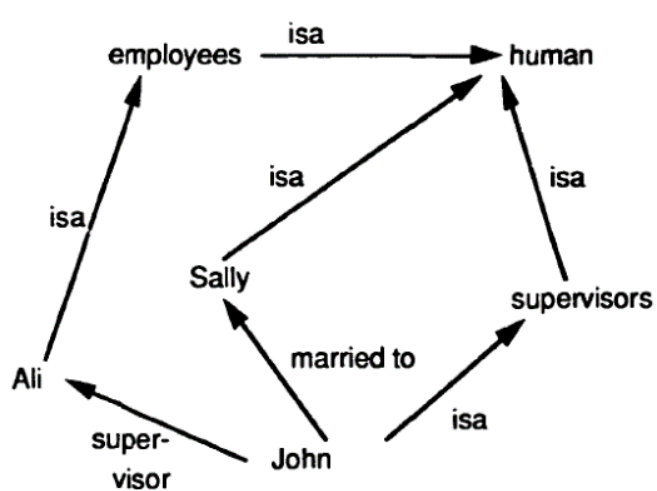
\includegraphics[width=0.45\textwidth]{images/sn.png}
  }
  \caption{Graph with two panels}
  \label{f:graph1}
\end{figure}


\subsection{Subsection with references to figures and panels} 

As usual with LaTeX, it is easy to refer to a figure: see figure \ref{f:graph1}. It is possible to refer to a specific panel in a figure, for instance figure \ref{f:panel1} or figure \ref{f:panel2}. Its also possible to refer to the entire figure, for instance figure \ref{f:graph1} or figure \ref{f:graph2}. It is also possible to refer to a panel within a figure by itself, for instance panel \subref{f:panel1} or panel \subref{f:panel2} in figure \ref{f:graph1}.

\section{A section with cross-references}

As usual, it is possible to reference an equation, such as equation \eqref{e:cv}. It is also possible to reference a section, such as section \ref{s:graphs}.


\section{Conclusion}\label{s:ccl}

At vero eos et accusamus et iusto odio dignissimos ducimus, qui blanditiis praesentium voluptatum deleniti atque corrupti, quos dolores et quas molestias excepturi sint, obcaecati cupiditate non provident, similique sunt in culpa, qui officia deserunt mollitia animi, id est laborum et dolorum fuga. At vero eos et accusamus et iusto odio dignissimos ducimus, qui blanditiis praesentium voluptatum deleniti atque corrupti, quos dolores et quas molestias excepturi sint.

\bibliography{\bib}
\end{document}